\documentclass[a4paper, twocolumn]{article}

\usepackage[english]{babel}
\usepackage[utf8]{inputenc}

\usepackage{amssymb, amsmath}
\usepackage{physics}
\usepackage{graphicx, xcolor,dblfloatfix}
\usepackage{subcaption}
\usepackage{siunitx}
\usepackage{booktabs, caption}
% subfig,
%******RELAZIONE DOMINIO TEMPO*****

\graphicspath{def_graph}

\begin{document}

\title{Comparison between two oscillator}
\author{Stefano Pilosio}

\maketitle

\section{Abstract}

This report want to show the difference between two oscillating circuits that use only an operational amplifier, in particular the focus will be on the different functioning principle, the waveform produced, its quality and the electrical characteristic of the waveform, so frequency and voltage peak to peak.

\section{Introduction}

\subsection{Astable Multivibrator}


\begin{center}
    \centering
    \def \svgwidth{\columnwidth}
    \input{def_graph/Multivibrator.pdf_tex}
\end{center}

As shown in figure, the circuit is composed of two feedback loops, one gives positive feedback and the other negative feedback. Due to positive feedback in this circuit virtual ground principle cannot be used. In principle the circuit can be divided in two parts:

\begin{itemize}
    \item The Positive Feedback Loop, that behaves like a Schmidt Trigger.
    \item The Negative Feedback Loop, that due to the presence of the capacitor introduce a time constant and induces the oscillations.
\end{itemize}

To understand why it oscillates we must write KVL (Kirchhoff Voltage Law):
\begin{gather}
    \begin{cases}
        v_{out} - v^+ = R_2i_2\\
        v^+= R_1i_2\\
        v_{out}-v^- = R i\\
        C\dv{v^-}{t}= i\\
        v_{out} = E \cdot (v^+-v^-)
    \end{cases}\\
    \begin{cases}
        \label{eq:genStable}
        v^+=v_{out}\frac{R_1}{R_1+R_2}\\
        v^-=v_{out}-RC\dv{v^-}{t}\\
        v_{out} = E \cdot (v^+-v^-)
    \end{cases}
\end{gather}

In \eqref{eq:genStable}, it is necessary to divide in two complementary scenarios: the charge and discharge of a capacitor, in fact suppose the capacitor is charged with a positive voltage and \(v_{out}\) is negative, then first the capacitor will discharge that follows \(\dv{v^-}{t}= \frac{v_{V_out}}{RC}\exp\left(\frac{-t}{RC}\right)\), and then it will charge with \(\dv{v^-}{t}= \frac{v_{V_out}}{RC}\left(1-\exp\left(\frac{-t}{RC}\right)\right)\). In general, considering only the discharge, the condition where \(v_{out}\) switches from positive to negative is:
\begin{equation}
    \label{eq:trigCond}
    \exp\left(\frac{-t}{RC}\right) = \frac{R_2}{R_1+R_2}
\end{equation}

So from \eqref{eq:trigCond} is visible that the duration of an oscillation depends on \(\tau = RC\) but also on \(R_1\) and \(R_2\), that set the level of charge in the capacitor necessary to trig the Schmidt part of multivibrator.

\subsection{Colpitts Oscillator}

\begin{center}
    \centering
    \def \svgwidth{\columnwidth}
    \input{def_graph/Colpitts.pdf_tex}
\end{center}

As shown in figure this circuit is completely different from the previous one, in fact it uses only a negative feedback loop. In this case in the feedback loop we have an LC tank, consisting of two capacitors in series and an inductance in parallel. To start an oscillation it is necessary to respect the \emph{Barkhausen Criterion}, that states:

\begin{equation}
    G \ge \frac{1}{\beta}
\end{equation}

Where: \(G\) is the voltage gain of the OPAMP, and $\beta$ is the feedback ratio of the output. Another condition of the Barkhausen Criterion is the total shift phase of the loop must be an entire multiple of \(2\pi\). 
The feedback ratio is calculated as follows: 

\begin{gather}
        \beta  = \frac{X_{C_2}}{X_{C_1}} = \frac{\frac{1}{\omega_0 C_2}}{\frac{1}{\omega_0 C_1}} = \frac{C_1}{C_2}\\
    \frac{1}{\beta}= \frac{C_2}{C_1}
\end{gather}

So the resulting inequality is:

\begin{equation}
    G = \frac{R_f}{R_{in}} \ge \frac{C_2}{C_1}
\end{equation}

The only elements in the circuit that causes a phase shift are the capacitors, the inductance and the OPAMP. The latter is in an inverting configuration, so it gives the required $2\pi$, so to obtain an oscillation the sum of impedance of the passive components must be zero:

\begin{gather}
    X_l + X_{C_1}+X_{C_2}=0\\
    j2\pi fL -\frac{j}{2\pi fC_1} -\frac{j}{2\pi fC_2} = 0\\
    (2\pi f)^2 L = \frac{C_1+C_2}{C_1C_2}=\frac{1}{C_{eq}}\\
    f = \frac{1}{2\pi\sqrt{L\cdot C_{eq}}}  
\end{gather} 

\section{Measurement Methods}
% Sottosezione Strumenti di Misura
\subsection{Materials}
\subsubsection{Instruments}
\begin{itemize}
    \item Oscilloscope ``Tektronix TDS 1012B'';
    \item Function Generator ``Agilent 3322A'';
    \item Power Supply.
\end{itemize}
\subsubsection{Equipment}
\begin{itemize}
    \item OPAMP ``LT081'';
    \item Breadboard;
    \item Wires;
    \item Resistors;
    \item Capacitors;
\end{itemize}

\subsection{Procedure}

After assembling the circuits on a Breadboard, it was applied a constant negative and positive voltage of \SI{15}{\volt} on the alimentation pins of OPAMP. Then in both case an oscilloscope probe was connected on the output, in the case of the multivibrator a second probe was connected across the capacitor.  Then via OSC, the waveforms were sampled and saved on an Excel file in the lab computer. 
Then the capacitor was swapped (in Colpitts case only $C_1$ capacitor was swapped) and the procedure was repeated.

\section{Analysis}

To analyze the circuit it was used a python environment that uses the libraries ``\emph{NumPy, Pandas and Matplotlib}'' in a Jupyter Notebook. 


\subsection{Frequency}

The analysis done was to determine the oscillation frequency, in both circuits a capacitor was changed across several values to see the change in frequency and different waveform.

The sampled waveforms consist of 2500 points, this points in the program are collected in a NumPy array and then are passed in NumPy's FFT algorithm, this algorithm returns a complex valued array, representing the Fourier Transform of the circuit, to obtain the fundamental frequency it is calculated the modulus of the component of the array and from it are extracted the highest value.

From this we can confront the value with the expected value in both cases, and also we can confront how \emph{good} is the produced waveform with the expected waveform confronting the harmonics of the two.

\subsection{Astable Multivibrator}

Because there are a lot of graphs, they are inserted in appendix~\ref{app:multivib}.

In the case of the Multivibrator the simulation are not consistent with the sampled results, this is probably due to a human error, in fact the resistance used are all \SI{10}{\kilo\ohm}, but probably the capacitance values are mislabelled, another error made is that the point where the probes were connected is not consistent, in fact the probe were connected. Even so some consideration can be made, in fact the only consistent measure is taken in point $v^+$, it is possible to see from the graphs that the amplitude of the signal in  is effectively limited from the resistive voltage divider to \SI{7.5}{\volt}, which correspond effectively to half $V_{cc}$ which was \SI{15}{\volt}.

Another thing that can be seen is in the graphs where the voltage is taken in $v^+$ and $v^-$ is that the effective switch of the voltage is in correspondence of $v^-\approx v^+$. Instead, in graphs where the points taken are $v_{out}$ and $v^+$ it is possible to denote that the output wave is not perfect.

Other considerations that can be made are on the frequency, in fact it is clearly visible that it has a correlation to the capacitance used, also in the circuit with the highest frequency it is observable the slew rate of the OPAMP, it is due to a limitation to the maximum output current of the OPAMP, that limits the maximum voltage variation supported by the OPAMP, it is a form of distortion and in some case can introduce a difference in phase.

% \begin{center}
%     \begin{tabular}
%         \toprule
%         {Capacitance} & {Frequency}\\
%         {\si{\farad}} & {\si{\hertz}}\\
%         \midrule
%         \num{1.5e-3} &\\
%         \num{150e-6} & \\
%         \num{730e-9} & \\
%         \num{955e-12}& \\
%         \bottomrule
%     \end{tabular}
% \end{center}


\subsection{Colpitts Oscillator}

Because there are a lot of graphs, they are inserted in appendix~\ref{app:colpitts}.


The common parameters for this experiment are the Inductance $L$ (value : \SI{200}{\micro\henry}) and $C_2$ (value : \SI{1}{\nano\farad})

It is clearly visible that this oscillator produces sinusoidal waves at high frequency, in fact in most cases the FFT produces a peak in the frequency of the wave, this is expected from the Fourier Transform of a Sinusoidal wave, in fact it is a Dirac Delta centered in the peak frequency.


\begin{table}[h]
    \caption{The measured frequency in relation to the capacitance used in $C_1$}
    \begin{tabular}{SSS}
        \toprule
        {Capacitance $C_1$} & {Expected Frequency} & {Frequency} \\
        {(\si{\farad})} & {(\si{\hertz})} & {(\si{\hertz})}\\
        \midrule
        \num{47e-9}  & \num{360e3} & \num{200e3}\\
        \num{470e-12}& \num{630e3} & \num{250e3}\\
        \num{560e-12}& \num{590e3} & \num{600e3}\\
        \num{635e-12}& \num{570e3} & \num{550e3}\\
        \num{10e-9}  & \num{370e3} & \num{400e3}\\
        \bottomrule
    \end{tabular}
\end{table}
\section{Conclusion}

It can be seen, even if only a qualitative way that the two oscillators produce in most cases the desired waveform, even if of two completely different types. The Astable Multivibrator can produce very low frequency waves without distortion, but at high frequency is limited by the properties of the OPAMP used. Instead, Colpitts Oscillator produces with low distortion waves at very high frequency, its only defects are in the choice of components that must respect the criteria. Another very important point is in the measure of the value of the components, in fact most electrical components are very similar, so it is important to keep track of the value used. 

\appendix
\onecolumn
\section{Astable Multivibrator Graphs}
\label{app:multivib}

% \begin{figure}[t]
%     \centering
% \end{figure}

\begin{figure}[h!]
    \subfloat
    [In red the voltage in $v^+$, in blue $v_{out}$. In this case the blue waveform is effectively the output, the high level reached is due to the sum of the voltage across the capacitor and the output, in fact it is visible in the peak the capacitor discharge.]
    {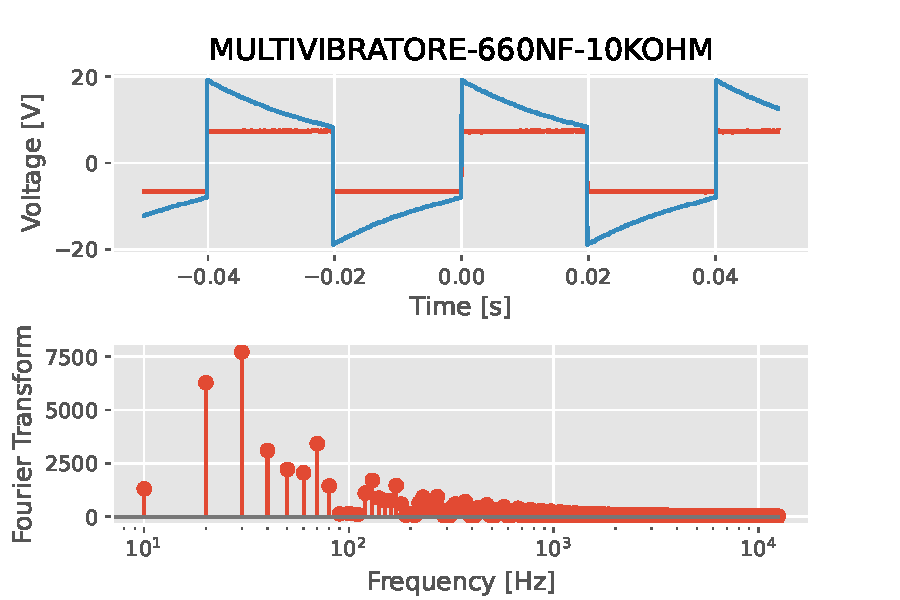
\includegraphics[width = .45\textwidth]{def_graph/MULTIVIBRATORE-660NF-10KOHM.pdf}} \qquad
    \subfloat
    [In red the voltage in $v^+$, in blue $v^-$, it is very visible in this case that the switch in the output happens when the capacitor voltage reaches the level set by the resistive voltage divider.]
    {%
        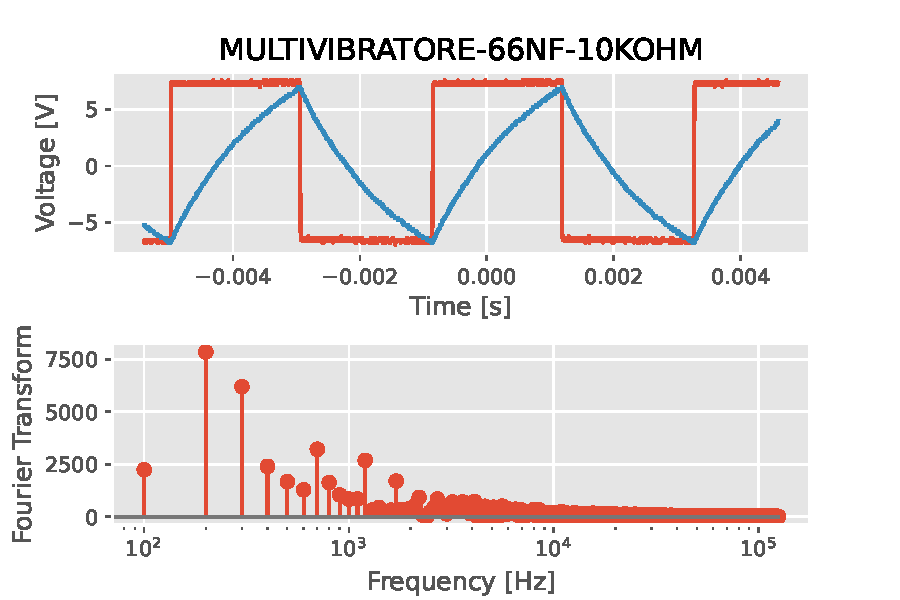
\includegraphics[width = .45\textwidth]{def_graph/MULTIVIBRATORE-66NF-10KOHM.pdf}%
        %
    }\\
    \subfloat
    [In red the voltage in $v^+$, in blue $v_{out}$.]%
    {%
        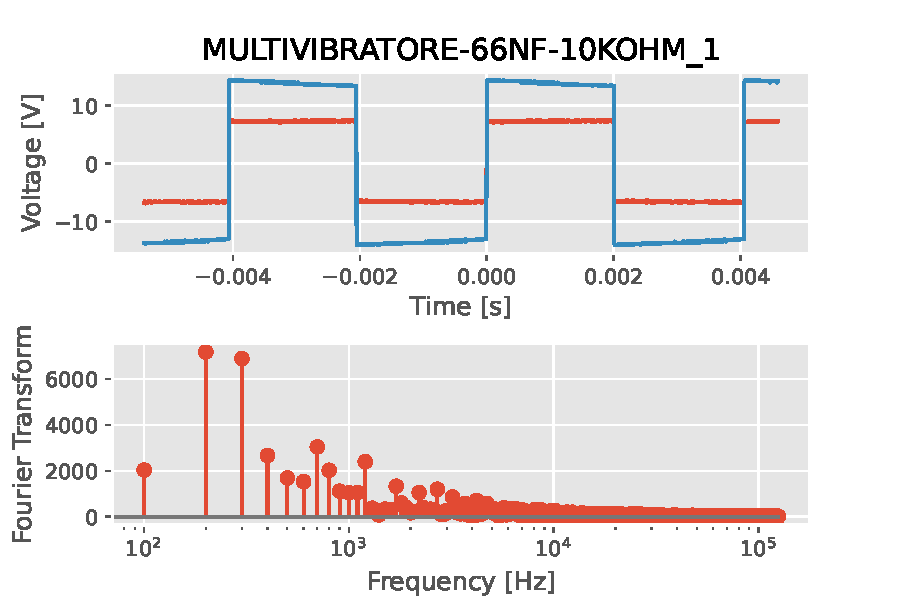
\includegraphics[width = .45\textwidth]{def_graph/MULTIVIBRATORE-66NF-10KOHM_1.pdf}%
    }\qquad
    \subfloat
    [In red the voltage in $v^+$, in blue $v^-$.]%
    {
        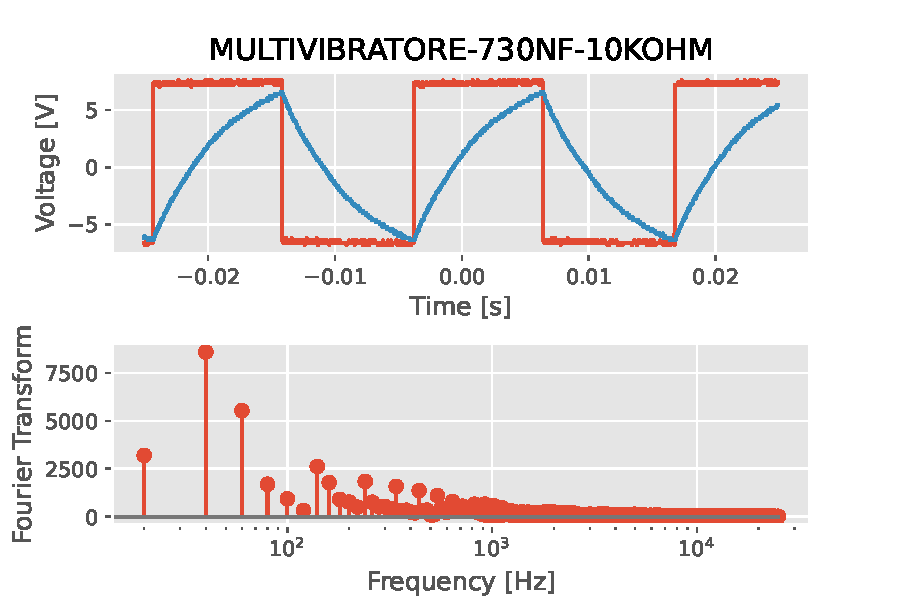
\includegraphics[width = .45\textwidth]{def_graph/MULTIVIBRATORE-730NF-10KOHM.pdf}%
    }\\
    \subfloat
    [In red the voltage in $v^+$, in blue $v^-$. In this graph is observable the distortion induced by the slew rate of the OPAMP.]%
    {%
        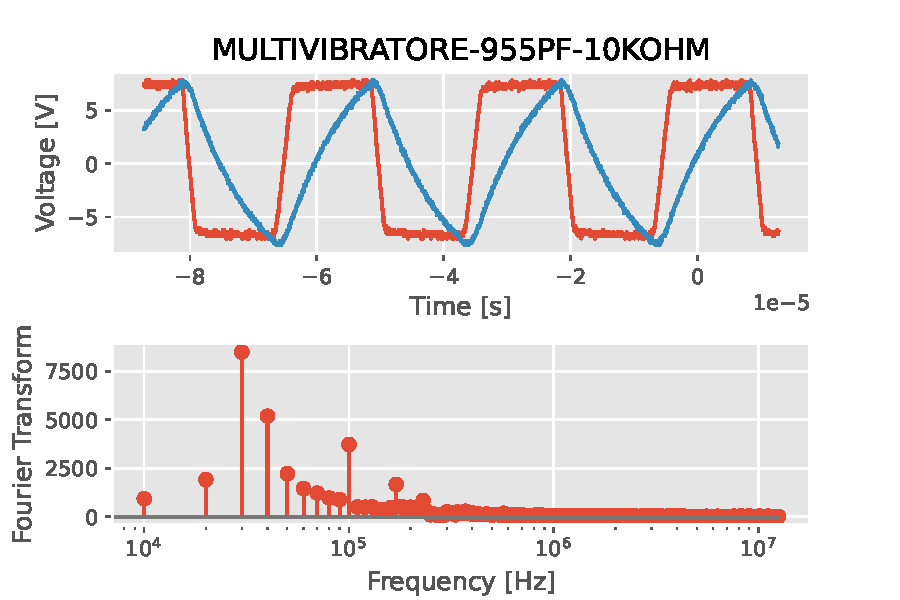
\includegraphics[width = .45\textwidth]{def_graph/MULTIVIBRATORE-955PF-10KOHM.pdf}%
    }
\end{figure}

\pagebreak

\section{Colpitts Oscillator Graphs}
\label{app:colpitts}

\begin{figure}[h!]
    \centering
    \subfloat{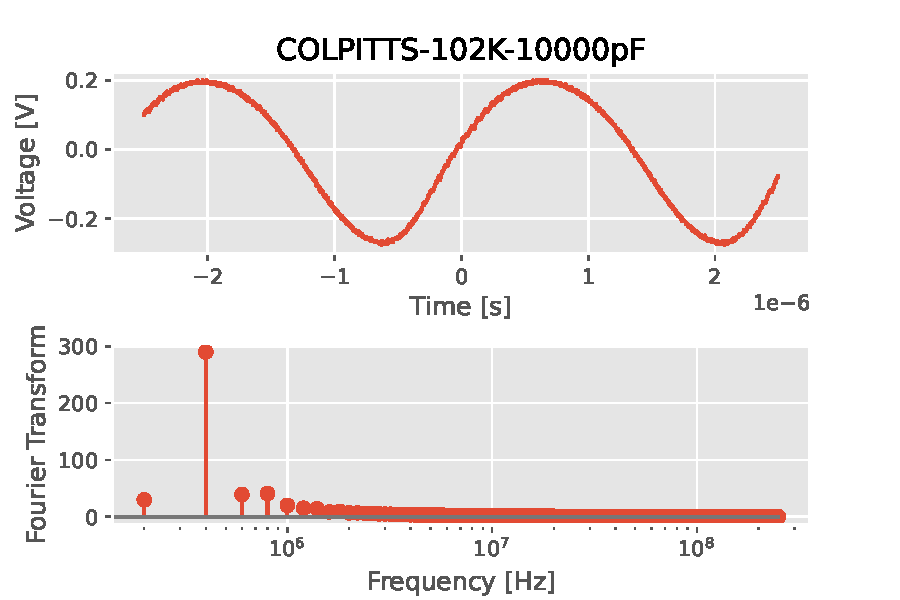
\includegraphics[width = .5\columnwidth]{def_graph/COLPITTS-102K-10000pF.pdf}}
    \subfloat[This is the sample with the highest frequency that maintains a perfect sinusoidal waveform]{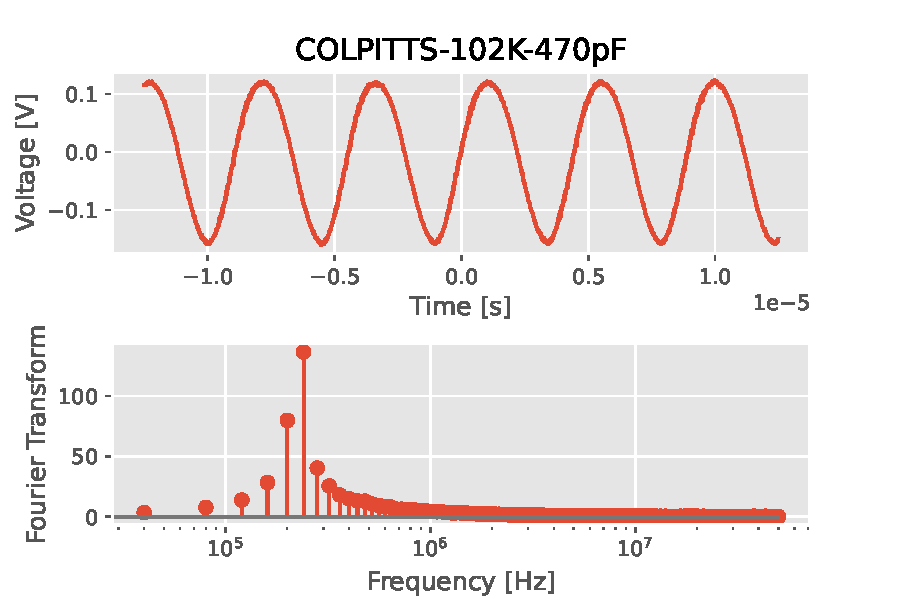
\includegraphics[width = .5\columnwidth]{def_graph/COLPITTS-102K-470pF.pdf}}\\
    \subfloat{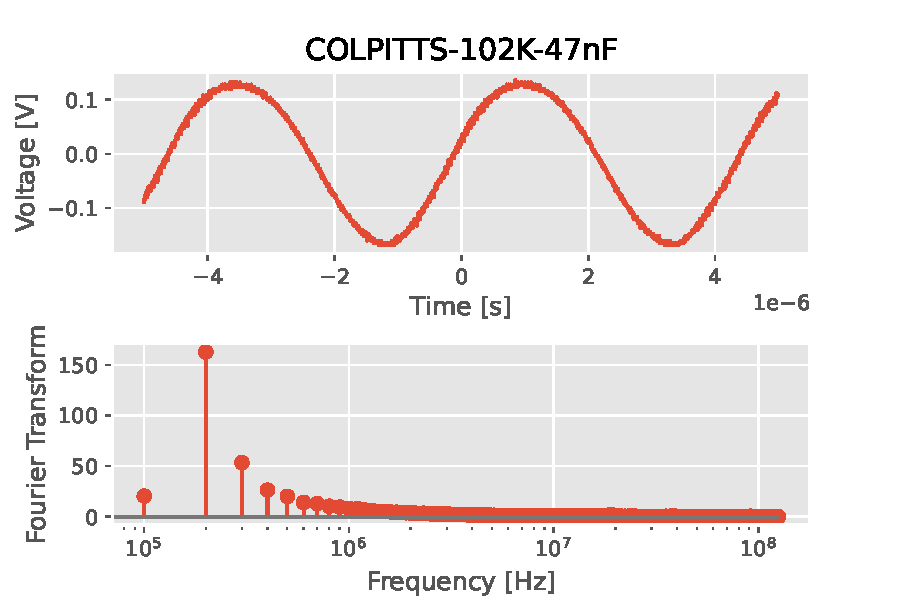
\includegraphics[width = .5\columnwidth]{def_graph/COLPITTS-102K-47nF.pdf}}
    \subfloat[In this case is visible dome distortion]{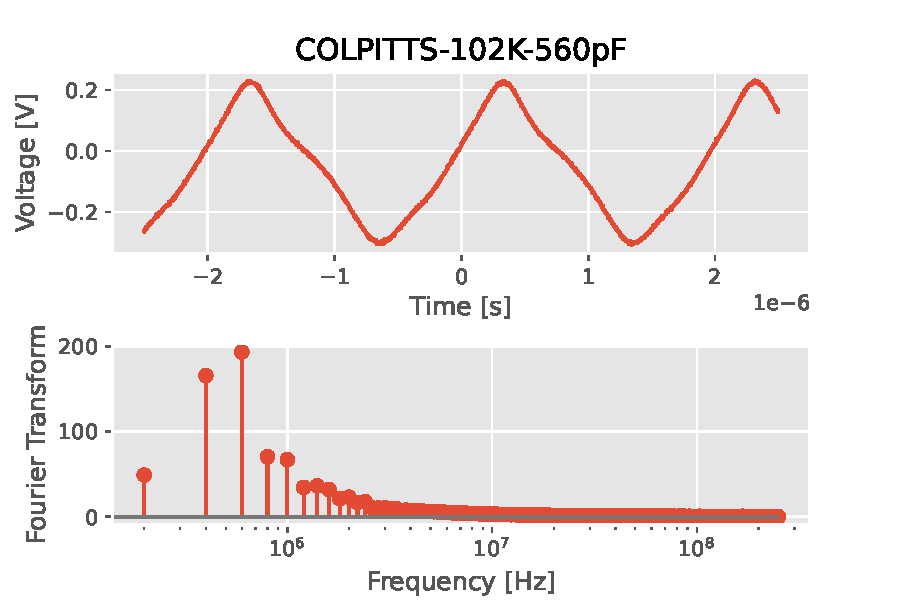
\includegraphics[width = .5\columnwidth]{def_graph/COLPITTS-102K-560pF.pdf}}\\
    \subfloat[Also in this case distortion is present]{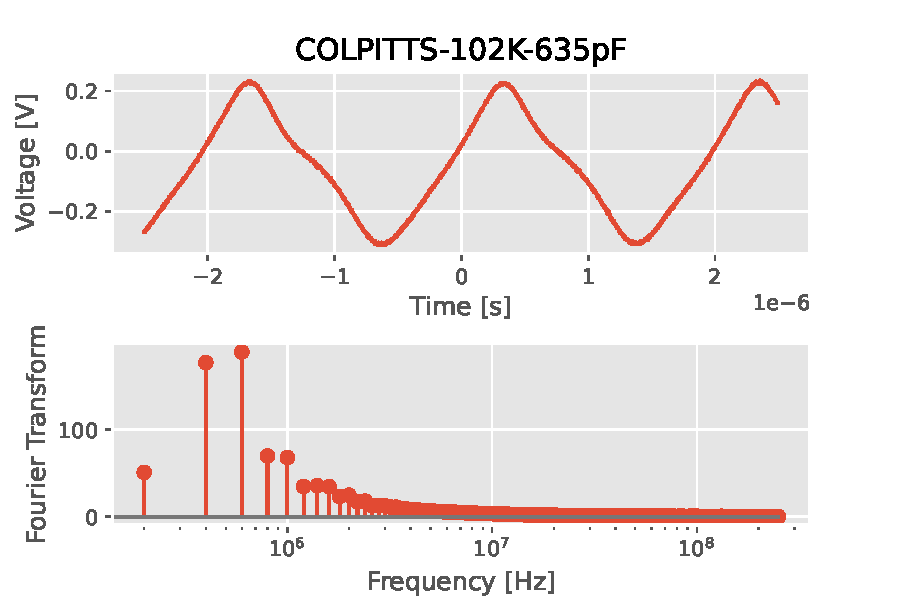
\includegraphics[width = .5\columnwidth]{def_graph/COLPITTS-102K-635pF.pdf}}
\end{figure}

\end{document}